\section{One scalar recovers all projective lines}\label{sec:lines}

The intersection calculation produces a power correction for two points at
a time.  We now show that a single correction works throughout the
projective space.  The passage from local power corrections to a global
one parallels \citet[Section~3.5]{CadoretPirutka2021}; here the degree-$p$
subfields give a particularly simple connected graph on which to propagate
the correction.

We first record why a nontrivial scalar cannot preserve projective lines.
This will rule out a new scalar when we apply the line-recovery argument
to the inverse map.

\begin{lemma}\label{lem:scalar-line}
Let $F$ have characteristic $p$, with $F\ne F^p$.  If multiplication by
$r\in\Fp^\times$ on $V_F$ maps every projective line over $F^p$ into a
projective line, then $r=1$.
\end{lemma}
\begin{proof}
Represent $r$ by an integer $1\le r<p$ and take $x\in F\setminus F^p$.
The points $[1],[x],[x+1]$ lie on one line.  Their images under
multiplication by $r$ are $[1],[x^r],[(x+1)^r]$.  The first two are
distinct, so the asserted line containment implies
\[
 (x+1)^r\in F^p+F^p x^r.
\]
If $1<r<p$, the binomial expansion has nonzero coefficient $r$ at
$x^{r-1}$.  This contradicts the linear independence of
$1,x,\ldots,x^{p-1}$ over $F^p$ from Lemma~\ref{lem:p-basis}.
\end{proof}

\begin{proposition}\label{prop:lines}
Let $K/k$ and $L/l$ be finitely generated extensions of algebraically
closed fields of characteristic $p$, both of transcendence degree at
least two.  For every compatible isomorphism $\Theta:V_K\to V_L$, there
is a unique $n\in\Fp^\times$ such that $\Psi=n\Theta$ sends every
projective line over $K^p$ onto a projective line over $L^p$.
\end{proposition}
\begin{proof}
Put $H=K^p$ and $C=L^p$.  We first find one scalar for which lines map
into lines.  Only after this construction will we apply it to the inverse.

\smallskip
\noindent\emph{A connected graph of independent image pairs.}
On the nonzero elements of $V_K$, join $[x]$ and $[y]$ by an edge when
\[
 C(X)\ne C(Y),\qquad [X]=\Theta([x]),\quad [Y]=\Theta([y]).
\]
This condition is independent of the chosen representatives.  Since
$X,Y\notin C$, the fields $C(X)$ and $C(Y)$ have degree $p$ over $C$.
An edge therefore means that $X,Y$ are $p$-independent.
The graph is complete between distinct parts of the partition by the
fields $C(X)$.  It has at least two parts: by Lemma~\ref{lem:p-degree},
$[L:C]\ge p^2$, so for any $X\notin C$ there is an element of
$L\setminus C(X)$, and $\Theta$ is surjective.  Thus every vertex has a
neighbor, and any two vertices are joined by a path of length at most two.

\smallskip
\noindent\emph{An affine configuration along an edge.}
Fix an edge $[x],[y]$.  The elements $1,x,y$ are linearly independent
over $H$.  Indeed, a dependence would give $y=c+dx$ with $c,d\in H$
and $d\ne0$, since $x,y\notin H$.  If $c=0$, the two vertices would
coincide.  Otherwise Lemma~\ref{lem:affine-symbol} gives
$\{x,y\}_K=0$, and compatibility followed by
Lemma~\ref{lem:zero-symbol} gives $Y\in C(X)$, again contradicting
the edge condition.

For arbitrary $a,b\in H^\times$, set
\begin{equation}\label{eq:affine-configuration}
 u=x+a,\qquad v=y+b,\qquad z=bx-ay=bu-av.
\end{equation}
These are nonzero: $u,v$ are nonzero because $x,y\notin H$, and
$z\ne0$ because $x,y$ are $H$-linearly independent.  Moreover,
\begin{equation}\label{eq:nonmonomial-source}
 [u]\notin\Fp[x],\qquad [v]\notin\Fp[y].
\end{equation}
For example, $[u]=i[x]$ with $0\le i<p$ would give
$x+a=h x^i$ for some $h\in H^\times$, contrary to the linear
independence of $1,x,\ldots,x^{p-1}$ and the condition $a\ne0$.
Figure~\ref{fig:affine-configuration} shows the incidence that explains
the two expressions for $z$.

\begin{figure}[htbp]
\centering
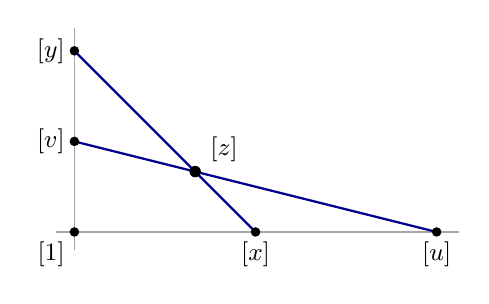
\begin{tikzpicture}[scale=1.15,every node/.style={font=\small}]
 \coordinate (O) at (0,0);
 \coordinate (x) at (2,0);
 \coordinate (u) at (4,0);
 \coordinate (y) at (0,2);
 \coordinate (v) at (0,1);
 \coordinate (z) at (1.333333,.666667);
 \draw[gray!70] (-.2,0)--(4.25,0);
 \draw[gray!70] (0,-.2)--(0,2.25);
 \draw[blue!55!black,thick] (y)--(x);
 \draw[blue!55!black,thick] (v)--(u);
 \fill (O) circle (1.5pt) node[below left] {$[1]$};
 \fill (x) circle (1.5pt) node[below] {$[x]$};
 \fill (u) circle (1.5pt) node[below] {$[u]$};
 \fill (y) circle (1.5pt) node[left] {$[y]$};
 \fill (v) circle (1.5pt) node[left] {$[v]$};
 \fill (z) circle (1.8pt) node[above right,xshift=2pt] {$[z]$};
\end{tikzpicture}
\caption{The source configuration in the projective plane
$\PP_H(H+Hx+Hy)$.  The point $[z]$ lies on both the line joining
$[x],[y]$ and the line joining $[u],[v]$.  The drawing records only
incidences; it imposes no order or metric on the characteristic-$p$
field.}
\label{fig:affine-configuration}
\end{figure}

Lemma~\ref{lem:affine-symbol}, applied also to
$z/x=b-a(y/x)$ and $z/u=b-a(v/u)$, gives
\begin{equation}\label{eq:configuration-symbols}
 \{x,u\}_K=\{y,v\}_K
 =\{y/x,z/x\}_K=\{v/u,z/u\}_K=0.
\end{equation}
Write $[U]=\Theta([u])$, $[V]=\Theta([v])$, and
$[Z]=\Theta([z])$.  Compatibility and
Lemma~\ref{lem:zero-symbol} applied to the first two symbols show that
\[
 U\in C(X)^\times,\qquad V\in C(Y)^\times.
\]
Linearity and injectivity transport \eqref{eq:nonmonomial-source} to
$[U]\notin\Fp[X]$ and $[V]\notin\Fp[Y]$.
In particular $U,V\notin C$.  Also $Y/X\notin C$, since $X,Y$ are
$p$-independent, and $V/U\notin C$: otherwise $U$ would belong to
$C(X)\cap C(Y)=C$.  We may therefore apply
Lemma~\ref{lem:zero-symbol} to the last two symbols in
\eqref{eq:configuration-symbols}.  The result is
\[
 Z\in X C(Y/X)^\times\cap U C(V/U)^\times.
\]
All hypotheses of Proposition~\ref{prop:intersection} now hold.  It
gives a common integer $1\le n<p$ such that
\begin{equation}\label{eq:local-line-powers}
 U^n\in C+C X^n,\qquad V^n\in C+C Y^n,
\end{equation}
and either inclusion uniquely determines $n$.

\smallskip
\noindent\emph{Propagation of the scalar.}
Fix representatives for all vertices and their images.  For a vertex
$[x]$, fix one neighbor $[y]$ and one $b\in H^\times$.  As
$a\in H^\times$ varies, Proposition~\ref{prop:intersection} applies
to \eqref{eq:affine-configuration}.  The second inclusion in
\eqref{eq:local-line-powers}, whose pair $Y,V$ stays fixed, forces
the same $n$ for every $a$.  To compare choices of neighbor and $b$,
specialize to $a=1$, keeping $X$ and a representative $U$ of
$\Theta([x+1])$ fixed.  Uniqueness for the first inclusion shows that
these choices cannot change $n$.  Thus each vertex has a
well-defined scalar.  Adjacent vertices have the same scalar by
\eqref{eq:local-line-powers}.  Connectedness consequently supplies a
single $n$ for all vertices and all $a\in H^\times$.

Set $\Psi=n\Theta$, with $n$ viewed in $\Fp^\times$.
The line joining $[1]$ and $[x]$ consists of those two points and
$[x+a]$ for $a\in H^\times$.  The first inclusion in
\eqref{eq:local-line-powers} says exactly that its image is contained
in the line joining $[1]$ and $[X^n]$.  Every projective line is a
multiplicative translate of one through $[1]$: multiply the line
joining $[s],[t]$ by $s^{-1}$.  Multiplication by a nonzero field
element is linear over the field of $p$-th powers, and $\Psi$ respects
the multiplicative group law.  Thus $\Psi$ maps every line into a line.

\smallskip
\noindent\emph{Equality of lines and uniqueness.}
Scalar multiplication preserves compatibility, since it scales the
tensor square by the nonzero scalar $n^2$.  Hence $\Psi^{-1}$ is
compatible.  Apply the construction just completed, with the fields
reversed, to obtain $r\in\Fp^\times$ for which $r\Psi^{-1}$ maps
lines into lines.  Its composition with $\Psi$ is multiplication
by $r$ on $V_K$ and has the same line-containment property.
Lemma~\ref{lem:scalar-line} forces $r=1$.
Thus both $\Psi$ and its inverse map lines into lines.  If
$\Psi(\ell)\subseteq\ell'$, choose a line $\ell''$ containing
$\Psi^{-1}(\ell')$.  Then
\[
 \ell\subseteq\Psi^{-1}(\ell')\subseteq\ell''.
\]
Two projective lines cannot properly contain one another, so
$\ell=\ell''$ and both inclusions are equalities.  Applying $\Psi$
gives $\Psi(\ell)=\ell'$.

Finally, if $m\Theta$ also sends lines onto lines, then
$(m\Theta)\circ\Psi^{-1}$ is multiplication by $mn^{-1}$ on
$V_L$ and preserves lines.  Another application of
Lemma~\ref{lem:scalar-line} gives $m=n$.
\end{proof}
